\newpage
\section{THIẾT KẾ HỆ THỐNG}

\subsection{Thiết bị sử dụng}

\begin{figure}[H]
    \centering
    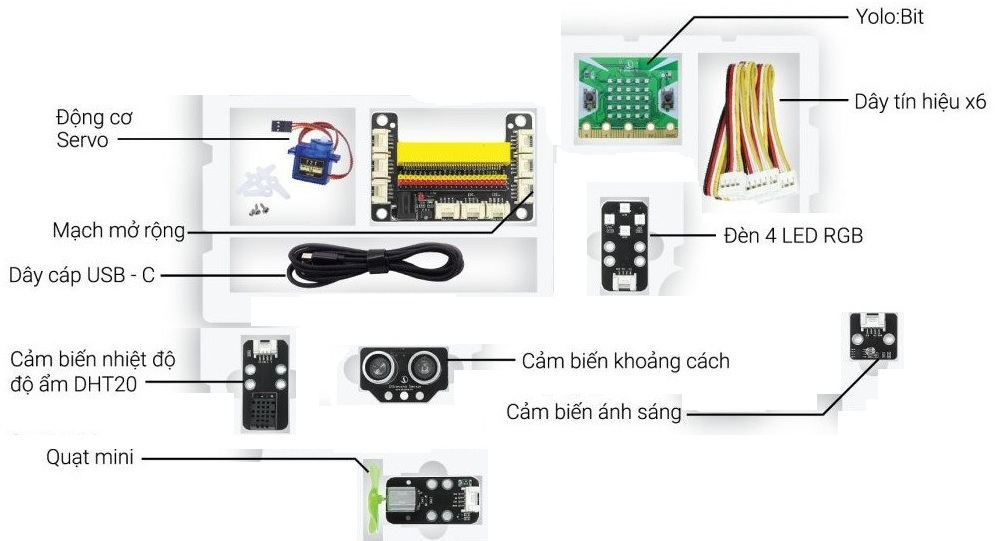
\includegraphics[width=\textwidth]{figures/selected_device.jpg}
    \caption{Thiết bị sử dụng trong hệ thống}
    \label{fig:selected_device}
\end{figure}

\textbf{Vi điều khiển và linh kiện kết nối}
\begin{itemize}
    \item \textbf{Yolo:Bit}: Vi điều khiển trung tâm, thực hiện thu thập dữ liệu từ các cảm biến và điều khiển các thiết bị đầu ra.
    \item \textbf{Mạch mở rộng}: Giúp mở rộng cổng kết nối, cấp nguồn và giao tiếp giữa Yolo:Bit và các thiết bị ngoại vi.
    \item \textbf{Dây tín hiệu (x6)}: Dây nối tín hiệu giữa Yolo:Bit và các cảm biến hoặc thiết bị điều khiển.
    \item \textbf{Dây cáp USB-C}: Dùng để cấp nguồn và lập trình cho Yolo:Bit từ máy tính.
\end{itemize}

\textbf{Thiết bị đầu vào}
\begin{itemize}
    \item \textbf{Cảm biến nhiệt độ độ ẩm DHT20}: đo nhiệt độ và độ ẩm môi trường; tự động kích hoạt quạt mini khi nhiệt độ vượt ngưỡng.
    \item \textbf{Cảm biến khoảng cách}: phát hiện vật thể ở khoảng cách nhất định, dùng để kích hoạt cảnh báo (như đèn LED RGB).
    \item \textbf{Cảm biến ánh sáng}: đo cường độ ánh sáng môi trường; tự động bật/tắt đèn LED RGB tùy vào điều kiện sáng/tối.
\end{itemize}

\textbf{Thiết bị đầu ra}
\begin{itemize}
    \item \textbf{Động cơ Servo}: điều khiển cơ cấu đóng/mở cửa hoặc chốt an toàn.
    \item \textbf{Đèn 4 LED RGB}: thể hiện trạng thái hệ thống (bình thường, cảnh báo, báo động).
    \item \textbf{Quạt mini}: kích hoạt khi nhiệt độ môi trường vượt ngưỡng để làm mát.
\end{itemize}

\begin{longtable}{|p{5cm}|p{4cm}|}
    \hline
    \textbf{Thiết bị}    & \textbf{Cổng kết nối} \\
    \hline
    Cảm biến ánh sáng    & P0                    \\
    \hline
    Cảm biến khoảng cách & P3 - P6               \\
    \hline
    Cảm biến DHT20       & I2C 1                 \\
    \hline
    Quạt mini            & P10                   \\
    \hline
    Đèn LED RGB          & P14                   \\
    \hline
    Động cơ Servo        & P4                    \\
    \hline
    \caption{Các thiết bị và cổng kết nối trên Yolo:Bit}
    \label{tab:devices}
\end{longtable}

\subsection{Mô tả hoạt động hệ thống}

\textbf{1. Luồng dữ liệu cảm biến}

\begin{itemize}
    \item \textbf{Cảm biến khoảng cách} kết nối qua các chân P3 đến P6 trên Yolo:Bit, dùng để phát hiện vật thể chuyển động hoặc người xâm nhập.
    \item \textbf{Cảm biến nhiệt độ/độ ẩm DHT20} sử dụng giao tiếp I2C (I2C 1) để đo các thông số môi trường.
    \item \textbf{Cảm biến ánh sáng} kết nối qua chân P0 để theo dõi cường độ ánh sáng môi trường.
    \item Yolo:Bit đọc dữ liệu từ các cảm biến, xử lý và gửi thông tin qua cổng USB-C tới máy tính qua giao tiếp Serial.
    \item Trên máy tính, một script Python hoạt động như một \textbf{IoT Gateway}, tiếp nhận dữ liệu từ Yolo:Bit, sau đó gửi lên Firebase (Realtime Database hoặc Firestore).
\end{itemize}

\textbf{2. Luồng điều khiển thiết bị}

\begin{itemize}
    \item Người dùng điều khiển hệ thống thông qua giao diện Web App, gửi lệnh (bật quạt, bật đèn, mở servo...) thông qua Firebase.
    \item Máy tính trung gian (IoT Gateway) đọc các dữ liệu từ Firebase, sau đó chuyển lệnh điều khiển đến Yolo:Bit thông qua cổng Serial.
    \item Yolo:Bit nhận lệnh và kích hoạt các thiết bị đầu ra tương ứng:
          \begin{itemize}
              \item \textbf{Quạt mini (P10)}: Bật khi nhiệt độ cao hoặc do người dùng điều khiển.
              \item \textbf{Đèn LED RGB (P14)}: Hiển thị trạng thái cảnh báo, báo động.
              \item \textbf{Động cơ Servo (P4)}: Điều khiển đóng/mở cửa hoặc khóa an toàn.
          \end{itemize}
\end{itemize}

\textbf{Sơ đồ khối kiến trúc hệ thống}

Hệ thống báo động an toàn gia đình sử dụng vi điều khiển \textbf{Yolo:Bit} để thu thập dữ liệu từ các cảm biến và điều khiển các thiết bị ngoại vi. Dữ liệu được xử lý cục bộ và đồng bộ hóa với giao diện web thông qua một máy tính trung gian (IoT Gateway) và dịch vụ \textbf{Firebase}.

\begin{figure}[H]
    \centering
    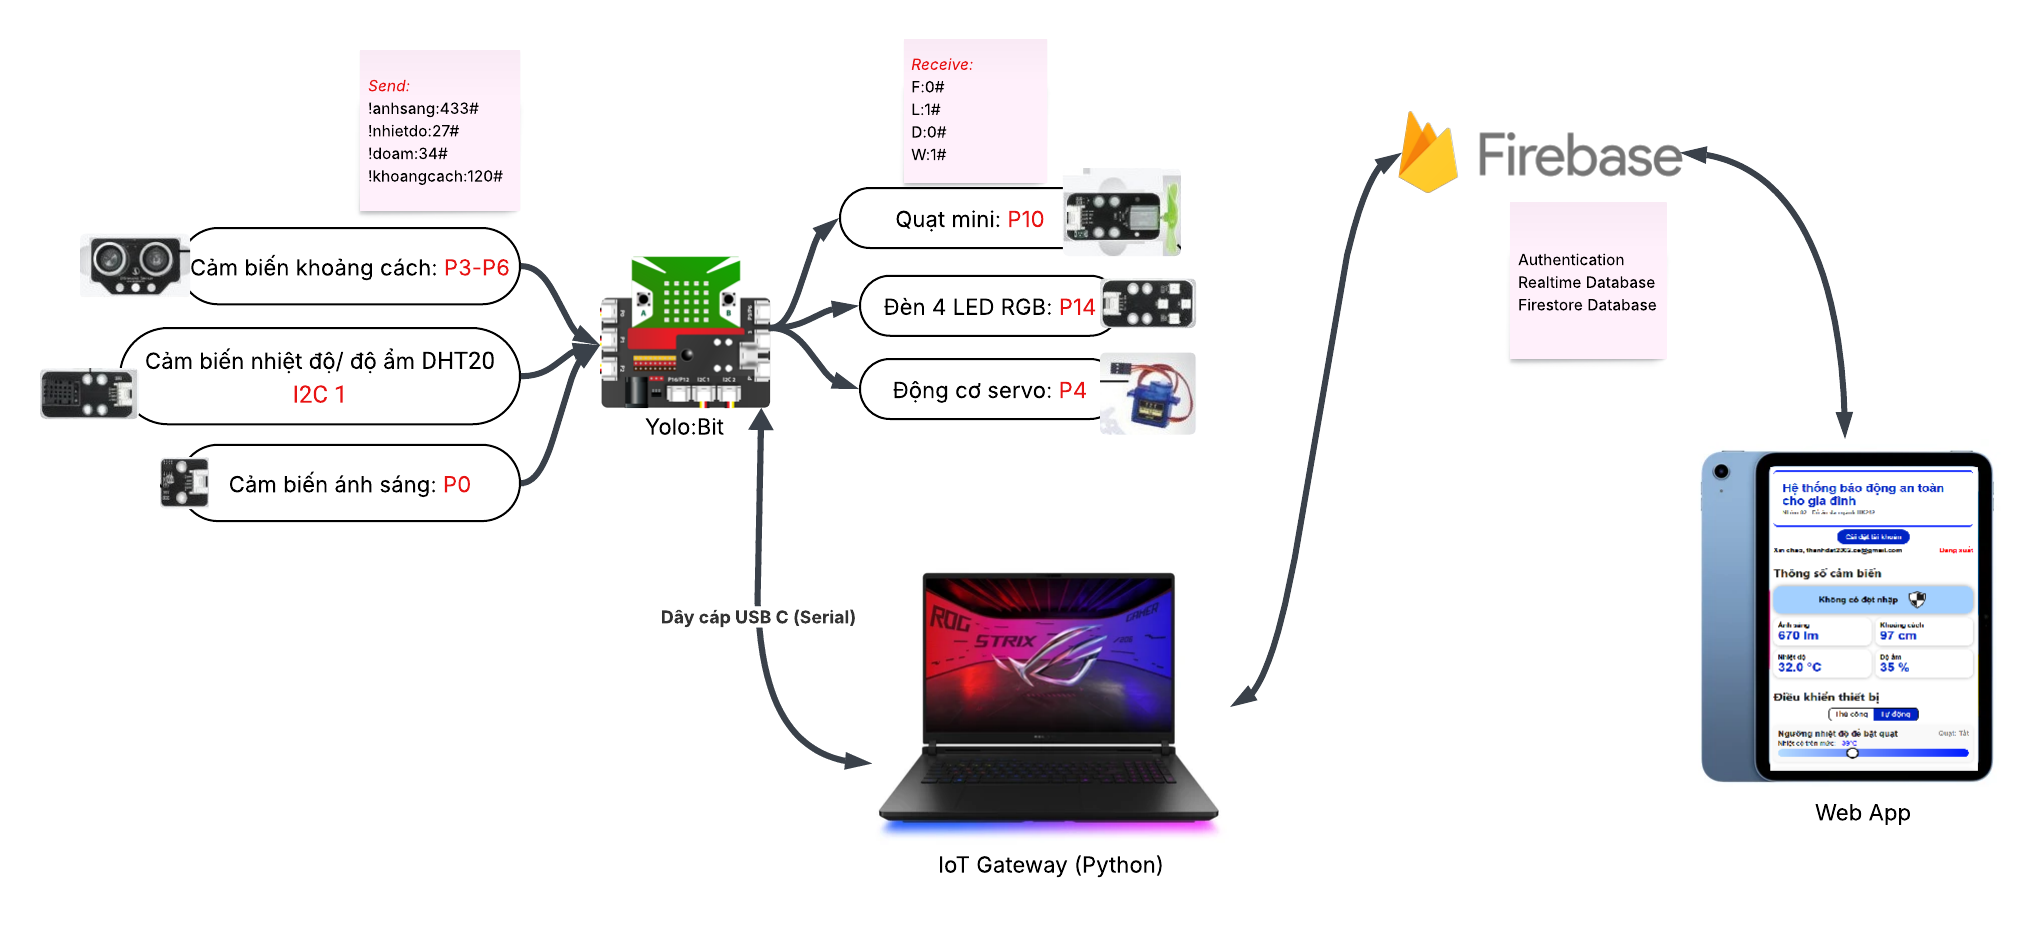
\includegraphics[width=\textwidth]{figures/tongquan.png}
    \caption{Sơ đồ khối kiến trúc hệ thống}
    \label{fig:tongquan}
\end{figure}


\begin{itemize}

    \item \textbf{Vi điều khiển trung tâm:} Yolo:Bit
          \begin{itemize}
              \item Đọc dữ liệu từ cảm biến
              \item Nhận/gửi dữ liệu qua Serial USB-C
              \item Kích hoạt thiết bị điều khiển theo lệnh từ Web
          \end{itemize}

    \item \textbf{Máy tính trung gian (IoT Gateway):}
          \begin{itemize}
              \item Nhận dữ liệu từ Yolo:Bit (Serial)
              \item Upload dữ liệu lên Firebase (Realtime DB hoặc Firestore)
              \item Nhận lệnh từ Firebase và chuyển về cho Yolo:Bit
          \end{itemize}


    \item \textbf{Firebase:}
          \begin{itemize}
              \item Authentication: xác thực người dùng
                    \begin{figure}[H]
                        \centering
                        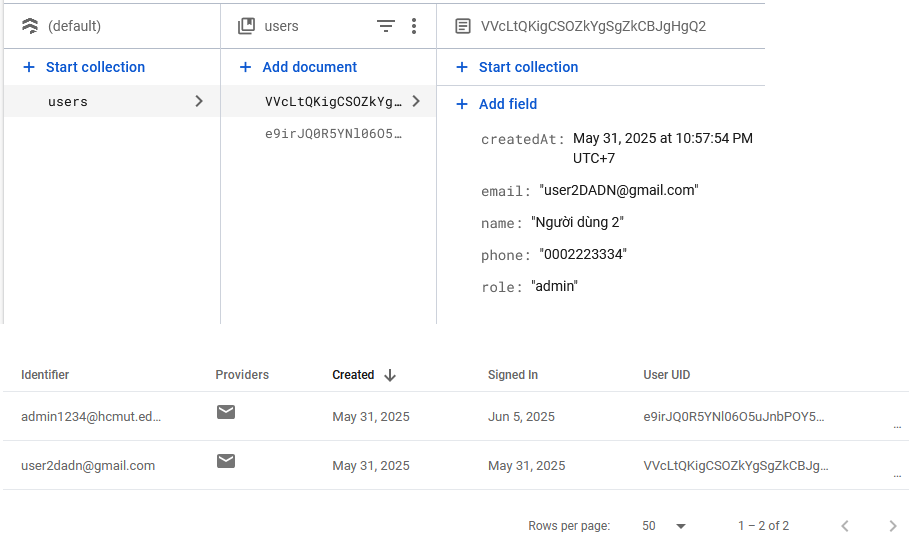
\includegraphics[width=0.7\textwidth]{figures/firebase2.png}
                        \caption{Cơ sở dữ liệu tài khoản người dùng trên Firebase}
                        \label{fig:firebase2}
                    \end{figure}
              \item Realtime Database / Firestore: lưu trữ dữ liệu cảm biến và điều khiển
                    \begin{figure}[H]
                        \centering
                        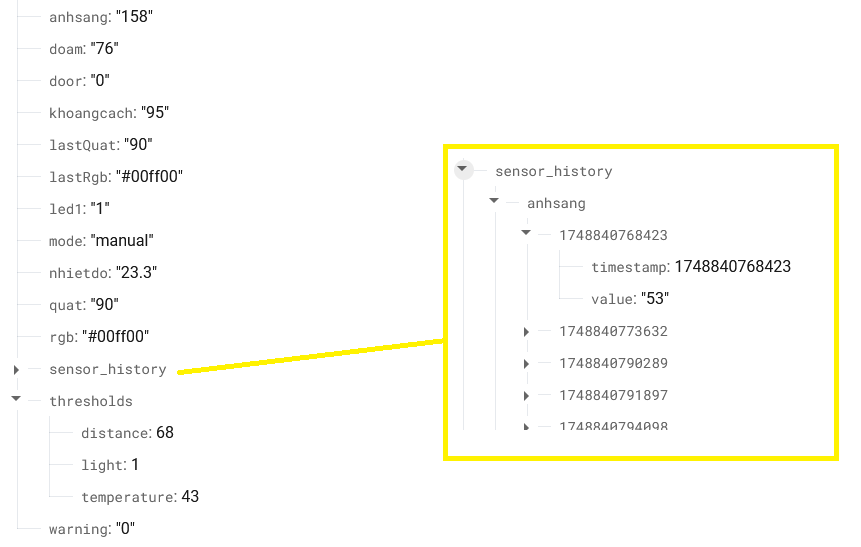
\includegraphics[width=0.7\textwidth]{figures/firebase1.png}
                        \caption{Lưu trữ dữ liệu và cài đặt hệ thống trên Firebase}
                        \label{fig:firebase1}
                    \end{figure}
          \end{itemize}



    \item \textbf{Web App:}
          \begin{itemize}
              \item Hiển thị thông tin cảm biến theo thời gian thực
              \item Gửi lệnh điều khiển thiết bị
              \item Cho phép người dùng đăng nhập và quản lý thiết bị, quản lý tài khoản
          \end{itemize}
\end{itemize}


\subsection{Công nghệ sử dụng}
\begin{itemize}
    \item \textbf{Firebase}: Xác thực người dùng và lưu trữ dữ liệu tài khoản, dữ liệu cài đặt và lịch sử dữ liệu môi trường.
    \item \textbf{Python (IoT Gateway)}: Quản lý giao tiếp với Yolo:bit và Firebase.
    \item \textbf{Công nghệ Web (HTML, CSS, JavaScript)}: Tạo giao diện người dùng để giám sát và điều khiển từ xa.
    \item \textbf{GitHub, GitHub Pages}: Lưu trữ mã nguồn và triển khai trang web.
\end{itemize}

Các công cụ khác:

\begin{itemize}
    \item \textbf{Figma, Photoshop}: Thiết kế giao diện cho Web App.
    \item \textbf{Lucidchart}: Vẽ các sơ đồ trong báo cáo.
    \item \textbf{Overleaf}: Soạn thảo và trình bày báo cáo.
\end{itemize}

\subsection{Sử dụng Design Pattern}

Trong quá trình xây dựng trang web điều khiển cho Hệ thống báo động an toàn, nhóm đã áp dụng một số mẫu thiết kế (\textit{Design Patterns}) để cấu trúc của hệ thống rõ ràng, dễ bảo trì hơn:

\begin{itemize}
    \item \textbf{Observer Pattern (Mẫu Quan sát viên)}:
          Ứng dụng trong việc cập nhật dữ liệu cảm biến và phản hồi hành động. Khi một cảm biến thay đổi giá trị (ví dụ: nhiệt độ tăng vượt ngưỡng), hệ thống sẽ tự động thông báo đến các thành phần liên quan (bật quạt). Giúp giảm sự phụ thuộc trực tiếp giữa các thành phần và tăng tính linh hoạt của hệ thống.

    \item \textbf{MVC Pattern (Model - View - Controller)}:
          Cấu trúc hệ thống web app và ứng dụng di động được thiết kế theo mô hình MVC. \textbf{Model} đại diện cho dữ liệu (cảm biến, thiết bị điều khiển), \textbf{View} là giao diện người dùng (giao diện web), và \textbf{Controller} xử lý logic trung gian như gửi lệnh từ người dùng đến thiết bị hoặc hiển thị dữ liệu cảm biến lên màn hình. Việc tách biệt ba thành phần này giúp dễ dàng thay đổi hoặc nâng cấp một phần mà không ảnh hưởng đến toàn bộ hệ thống.

    \item \textbf{Mediator Pattern (Mẫu Trung gian)}:
          Được sử dụng trong giao tiếp giữa các thiết bị thông qua máy tính trung gian (chạy Python script). Thay vì các cảm biến và thiết bị đầu ra giao tiếp trực tiếp với nhau, chúng đều kết nối và gửi nhận qua \textbf{Python script}, đóng vai trò trung gian quản lý luồng dữ liệu và lệnh điều khiển giữa các thành phần (Yolo:bit, Firebase, Web App). Giúp giảm độ phức tạp và tăng khả năng kiểm soát trung tâm.

    \item \textbf{Singleton Pattern}:
          Dùng Firebase như là \textbf{singleton service} để quản lý người dùng, quyền truy cập và cấu hình thiết bị. Trong toàn hệ thống, Firebase đóng vai trò độc nhất cho việc xác thực và lưu trữ cài đặt hệ thống, đảm bảo không có xung đột xảy ra giữa các phiên truy cập.
\end{itemize}

Dùng các Design Pattern giúp hệ thống có cấu trúc rõ ràng, dễ kiểm soát dòng dữ liệu và tăng cường khả năng mở rộng trong tương lai (tích hợp thêm các công nghệ AI, học máy hoặc hệ thống điều khiển phức tạp hơn).
